% !TEX TS-program = pdflatex
% !TEX encoding = UTF-8 Unicode

% This is a simple template for a LaTeX document using the "article" class.
% See "book", "report", "letter" for other types of document.

\documentclass[12pt]{article} % use larger type; default would be 10pt

\usepackage[utf8]{inputenc} % set input encoding (not needed with XeLaTeX)
\renewcommand\familydefault{\sfdefault}
\usepackage{helvet} 


%%% Examples of Article customizations
% These packages are optional, depending whether you want the features they provide.
% See the LaTeX Companion or other references for full information.

%%% PAGE DIMENSIONS
\usepackage[a4paper,landscape,twocolumn,margin=0.5in]{geometry} % to change the page dimensions
%\geometry{a4paper} % or letterpaper (US) or a5paper or....
%\geometry{margin=0.5in} % for example, change the margins to 2 inches all round
%\geometry{twocolumn} % two columns
%\geometry{landscape} % set up the page for landscape
%   read geometry.pdf for detailed page layout information

\setlength{\columnsep}{0.5in}

\usepackage{graphicx} % support the \includegraphics command and options
\usepackage{hyperref}

% \usepackage[parfill]{parskip} % Activate to begin paragraphs with an empty line rather than an indent

%%% PACKAGES
\usepackage{booktabs} % for much better looking tables
\usepackage{array} % for better arrays (eg matrices) in maths
\usepackage{paralist} % very flexible & customisable lists (eg. enumerate/itemize, etc.)
\usepackage{verbatim} % adds environment for commenting out blocks of text & for better verbatim
\usepackage{subfig} % make it possible to include more than one captioned figure/table in a single float
% These packages are all incorporated in the memoir class to one degree or another...

%%% HEADERS & FOOTERS
\usepackage{fancyhdr} % This should be set AFTER setting up the page geometry
\pagestyle{fancy} % options: empty , plain , fancy
\renewcommand{\headrulewidth}{0pt} % customise the layout...
\lhead{}\chead{}\rhead{}
\lfoot{}\cfoot{}\rfoot{\thepage}

%%% SECTION TITLE APPEARANCE
\usepackage{sectsty}
\usepackage{titlesec}
\allsectionsfont{\sffamily\mdseries\upshape\bfseries} % (See the fntguide.pdf for font help)
% (This matches ConTeXt defaults)

%%% END Article customizations

%%% The "real" document content comes below...

\title{\large{\vspace{-5ex}\textbf{Exploration and Modelling of Planetary Interiors}}\newline\\{\textbf{\underline{Lecture 12 - Giant Planet Formation}}}\vspace{-7ex}}
\author{}
\date{} % Activate to display a given date or no date (if empty),
         % otherwise the current date is printed 

\renewcommand*\contentsname{\large\textbf{Topics covered}\vspace{-2ex}}

\bibliographystyle{apalike}
\renewcommand\refname{Background reading}

\begin{document}
\begingroup
\let\center\flushleft
\let\endcenter\endflushleft
\maketitle
\endgroup

\begingroup
\let\cleardoublepage\relax
\let\clearpage\relax
\tableofcontents
%\listoffigures
%\listoftables
\endgroup

\begin{figure}[!htbp]
\begin{center}
 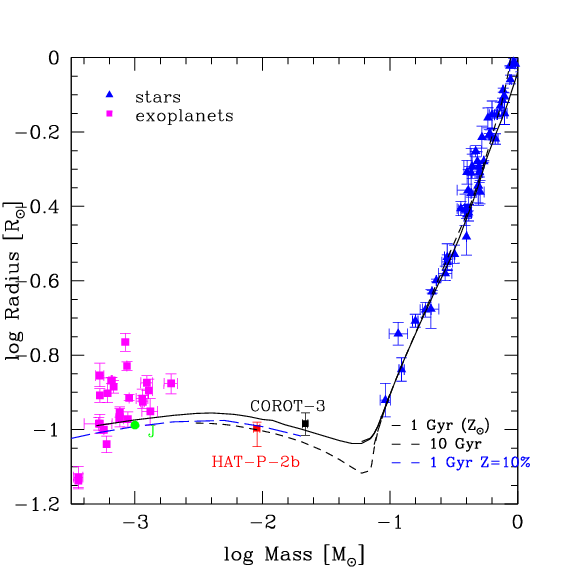
\includegraphics[width=0.99\textwidth,keepaspectratio=true]{./images/physics_stackexchange_com_questions_165283_gas_giant_six_times_more_massive}
 \caption{Apollo 12 landing site from LRO NAC}
 \label{A12_zoom_nomenclature}
\end{center}
\end{figure}

\section{Introduction}\vspace{-2ex}\titlerule[1pt]\bigskip

There are four giant planets in the solar system, Jupter, Saturn, Uranus and Neptune. The first two are called \textbf{gas giants} and the two other \textbf{ice giants}, due to their physics and their major constituting elements. Gas giants are mostly NH$_3$, CH$_4$ and H$_2$O, while ice giants are mostly H and He, and further away from the Sun.\newline\linebreak
It is worth mentioning here that giant planets are not limited to those, since the exoplanets search has started, many were found. These type where the first planets detected because of their sizes. Still now they are the most numerous found. New sub-types have been defined from the exoplanet discoveries, including closely orbiting \textbf{hot Jupiters} or \textbf{hot Neptunes}. The exoplanet search will certainly bring many more exotic samples to permit a better understanding of their population and especially their limits (when a giant is a brown dwarf, and vice-versa).\newline\linebreak
There are actually three different school of thoughts, and thus types of models that are built and tested to learn more about giant planets formation. We will investigate each one of them separately and then look at what we have learnt.
\clearpage



\subsection{Stevenson details}\vspace{-1ex}\bigskip

\cite{stevenson1982formation}


\section{Models}\vspace{-2ex}\titlerule[1pt]\bigskip

\subsection{Theories of giant planet formation}\vspace{-1ex}\bigskip

Lissauer SETI talk 2009 (\href{https://www.youtube.com/watch?v=FAa7hb2bT\_g}{link})\newline 

3 general models: \\
- Core-nucleated accretion: big rocks accumulated gas\\
- Fragmentation during collapse: Planet forms like star\\
- Giant gravitational instability in Disk: Giant protoplanets\\

\subsection{Core-nucleated instability}\vspace{-1ex}\bigskip

\noindent The model proposed by \cite{pollack1996formation} is first defining planetesimal properties as a mass fraction of H$_2$O Ice, Rock and CHON (Carbon, Hydrogen, Oxygen and Nitrogen). Each having a density, a latent heat (+: endothermic like ice and rock \& -: exothermic like CHON) and a vaporisation temperature. It defines and simulates both the gas and the planetesimal accretion rates together. \newline

\subsection{Gas flow near planet}\vspace{-1ex}\bigskip

Detection of planet size in accretion disk from\cite{bate2003three}.\newline

\subsection{Jupiter growth: hydrodynamic \& thermal constraints}\vspace{-1ex}\bigskip

\cite{lissauer2009models}. First models of growth from Mars mass to Jupiter mass. Parameters: disk viscosity, surface density, planet properties.\newline
High viscocity disks, accretion is higher.

\subsection{Assignment details}\vspace{-1ex}\bigskip

This assignment is worth 20\% of the marks for this module. You are advised to start work on this assignment at the start of the module, so that you give yourself plenty of time to complete it. The deadline for submission will be April 25$^{th}$ 2016 (the anticipated date of the revision session for this module).\newline\linebreak
The subject of the lecture notes is a broad one, in which more than one model has been proposed. You should first assemble a set of published background material on the subject. You can use Google Scholar as a resource for finding articles (insert “Giant Planet Formation” as the topic). Alternatively, you can start with some of the references in a short review paper by D J Stevenson which can be found at the following website (\href{http://authors.library.caltech.edu/9922/1/STEaipcp04.pdf}{link}).\newline \linebreak
Once you have found your background material, you should consider what topics you are going to cover in your lecture notes. Remember that the lecture is about formation of giant planets, so you do not need to describe giant planets and their interiors in great detail. You will also need to illustrate your notes with suitable figures, which can be obtained either directly from the background reading, or which can often be found on the Web. Remember to refer to each of your figures in order in your text. You must have a list of references at the end of your notes.\newline\linebreak
Use the same general template that we have used for our lecture notes (landscape pages; Arial 14pt text), and please do not exceed 14 printed pages


\newpage
\bibliography{EMPI_L12}
\end{document}
